%%%%%%%%%%%%%%%%%%%%%%%%%%%%%%%%%%%%%%%%%%%%%%%%%%%%%%%%%%%%%%%%%%%
%                                                                 %
%                            CHAPTER ONE                          %
%                                                                 %
%%%%%%%%%%%%%%%%%%%%%%%%%%%%%%%%%%%%%%%%%%%%%%%%%%%%%%%%%%%%%%%%%%%

\chapter{INTRODUCTION}

\section{Definitions of Version} \label{sec:def}

Using the term `version' in the vernacular has become so pervasive that few documents formally define it.
Barkstrom describes versions as \textbf{homogeneous groupings} used to control, ``production volatility induced by changes in algorithms and coefficients as result of validation and reprocessing," \cite{Barkstrom2003}.
The \textbf{groupings} he mentions is a method of separating data objects such that they have similar scientific or technical properties.
In order to determine when these properties have changed, he leverages the \gls{nasa} Earth Science workflow model shown in Figure \ref{NASALevels}.
\begin{figure}
	\centering
	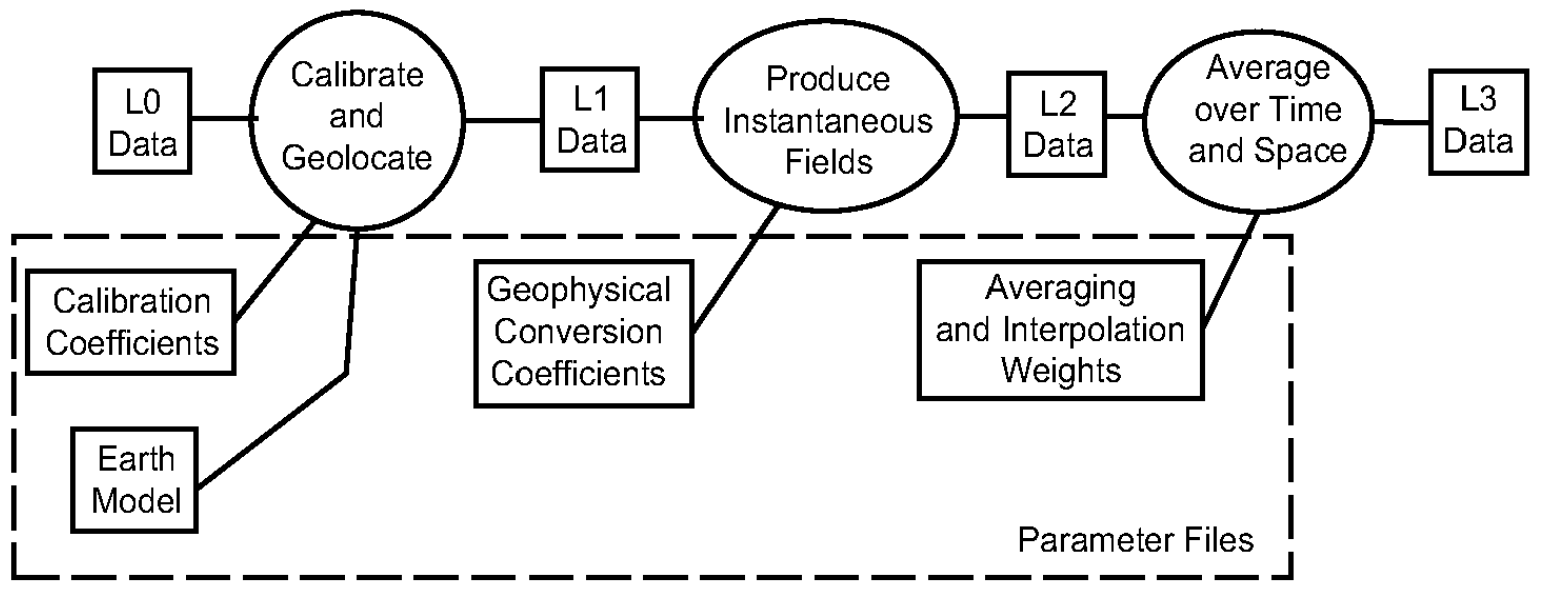
\includegraphics[scale=0.35]{figures/NASALevels.png}
	\caption[National Aeronautics and Space Administration Earth Science organizes its data into three levels depending on how much the data has been aggregated and processed from the original sensor measurements.]{National Aeronautics Space Administration Earth Science organizes its data into three levels depending on how much the data has been aggregated and processed from the original sensor measurements. Figure 1 from \cite{Barkstrom2003}}
	\label{NASALevels}
\end{figure}
The model describes the formal stages of processing to turn a raw remote sensing signal from satellite instruments into global aggregate summaries \cite{Barkstrom2003}.
The workflow model, therefore, describes a data object's \gls{provenance}, the information about how a piece of data or thing was created used to determine its quality, reliability or trustworthiness \cite{Moreau2013c}, not the version differences.
Provenance provides the mechanism to explain differences between \textbf{groupings} exposed by versioning activities.
Understanding the workflow model reveals that changes to either the algorithms or parameter files will force a change in the resulting data, creating a new version of the output data.
Each time the provenance changes, the levels take on a layer cake appearance as shown in Figure \ref{NASALayers}. 
\begin{figure}
	\centering
	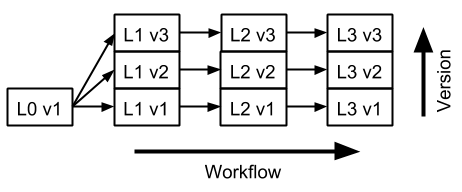
\includegraphics[scale=1]{figures/VersionLayerDiagram2.png}
	\caption[Versions Layered on the National Aeronautics and Space Administration Earth Science workflow model]{National Aeronautics and Space Administration Earth Science workflow model gains layers as changes to provenance induces version groupings to expand.  The new layer is homogeneous with other layers in the level, forming a grouping.  Level 0 cannot gain more layers because manipulating the source readings would invalidate the data.}
	\label{NASALayers}
\end{figure}
Unlike provenance, version information describes relations not along the workflow, but in an orthogonal direction.

The conflation can also be seen in \gls{linked} provenance models, Web of Data resources which describe the \gls{provenance} relating data sets, where version concepts and links are included into the ontology.
The \gls{prov} Ontology is the \gls{w3c} recommended method of documenting \gls{provenance} uses the property \textit{prov:derivation} to connect versions.
The \textit{prov:derivation}, covered more in Section \ref{sec:prov}, is defined as, ``a transformation of an entity into another, an update of an entity resulting in a new one, or the construction of a new entity based on a pre-existing entity," \cite{Lebo2013}.
The \gls{prov} definition establishes the existence of at least two distinct objects as a necessary condition for versioning.
An additional result of the \gls{prov} definition is that an object cannot be a version of itself.

Another definition comes from Tagger at the University College London on the versioning of biological data in which versions are a, ``semantically meaningful snapshot of a design object (an artifact) at a point in time," \cite{Tagger2005}.
He, unfortunately, does not further clarify what he means by semantically meaningful since the requirements to be meaningful varies based on the application.
He likely means that the design object must be complete or whole, interpretable in purpose by itself and not a subset.
The design object is used in the context of database objects, referring to an incomplete final product, and unifies the versions as their primary subject, capturing the object's state over the course of its design.

The \gls{ifla} formed a study group in February 1997 to, ``produce a framework that would provide a clear, precisely stated, and commonly shared understanding of what it is that the bibliographic record aims to provide information about, and what it is that we expect the record to achieve in
terms of answering user needs" \cite{frbr}.
A common problem in library sciences is the organization and documentation of multiple editions of a book or multiple translations of a book in a standardized manner.
A primary result of the group meeting is a standardized vocabulary to discuss distinct iterations of a literary work which follows strong parallels in data versioning.
The \gls{frbr} avoids the terms \textbf{edition} and \textbf{version} since ``those terms are neither clearly defined nor uniformly applied" \cite{frbr}.
Instead, they use the terms: \textbf{work}, \textbf{expression}, and \textbf{manifestation}.
A \textbf{work} refers to the abstract concept of a creative or artistic idea.
\textbf{Expressions} are then different forms of that particular \textbf{work}, embodying the most similar term to the previous definitions of versions.
A \textbf{manifestation} is the physical embodiment of an \textbf{expression}.
These three terms and their hierarchy establish a repeating theme throughout other versioning works.
The breakdown of terms identifies a need to differentiate between the granularity or scale of changes as differences in \textbf{works} are more significant than differences in \textbf{expressions}.
Models focused on versioning rather than provenance will also have a hierarchical structure as covered in Section \ref{sec:models}.

Combining these myriad of definitions, the Barkstrom definition provides the mechanism to detect and explain the source of a version.
The Tagger and \gls{prov} definitions explain the purpose of a version to expose differences between distinct objects.
The \gls{frbr} definition contextualizes a version as a more granular \textbf{expression} of a larger \textbf{work}.
The working definition in this dissertation of a \gls{version} is ``an \textbf{expression} of a \textbf{work} which exists in comparison to another object and communicates the extent to which it diverges from that object as a result of provenance changes".
Although each definition disagrees on the form a version object takes on, all but \gls{prov} derivation agree that a version belongs to a larger collection of objects implementing a more abstract, ideal representation.
Provenance provides the information necessary to explain ``semantically meaningful" for the Tagger definition as \textit{prov:Derivation} captures when a data object diverges into a new object.

\section{Why Versioning is Important}

\begin{quotation}
	``If scientific data production were easy, instruments would
	have stable calibrations and validation activities would discover no need for
	corrections that vary with time. Unfortunately, validation invariably shows that
	instrument calibrations drift and that algorithms need a better physical basis." \cite{Barkstrom2003}
\end{quotation}

Anyone who has used an iPhone or owned a video game console understands the basics of versioning.
Companies brand sequential devices to indicate improvements in performance or capabilities.
Basic numerical sequencing has given rise to a plethora of versioning systems used widely across a landscape of software and data.
Versioning systems help scientific workflows avoid losing work by managing transitions and changes while in operation \cite{Casati1996}.
Versioning systems provide necessary documentation which informs the transition to new methods and procedures \cite{Wiil:2000:RDH:338407.338517}.
Versioning systems provide accountability for the value of a project's data set when considering an agency's continued funding \cite{Cavanaugh2002}.
The natural evolution of versioning systems, however, have given rise to formal architecture operating on top of very informal concepts.
Disagreements between the informal concepts propagate through the formal architecture, causing breakdowns in interoperability between heterogeneous systems, especially when users are not aware of biases in informal versioning concepts \cite{Baker2009}.
In this dissertation, we identify gaps in versioning practices which result from tradition and develop a data model to more completely capture the interactions involved in versioning.

At the very core, versioning systems are a means of communication.
Data producers communicate to consumers how much the producer has changed the data.
The producer can also communicate through time using logs and other documentation.
In order to clearly communicate changes, ideas must be clearly formalized and defined and vice versa.

\section{Current Versioning Models} \label{sec:models}

Version models provide a visual theoretical aid in understanding where a data object lies in relation to the rest of a work.
The \gls{arm} group at Pacific Northwest National Laboratory used a model dividing the data into mathematical sets which versioning operations acted upon\cite{6906868}.
Adding files already in the set created a new set which inherited all non-intersecting files and included all the new ones.
The model provided a means to organize and automate the versioning of \gls{arm}'s daily expanding data sets.

The \gls{hcls} Interest Group of the \gls{w3c} recently released a model which resembles the \gls{frbr} model with a three level hierarchy of increasing granularity \cite{Dummontier2016}.
Their model, shown in Figure \ref{HCLSModel}, separates the concept of a data set into three groupings.
\begin{figure}%[b]
	\centering
	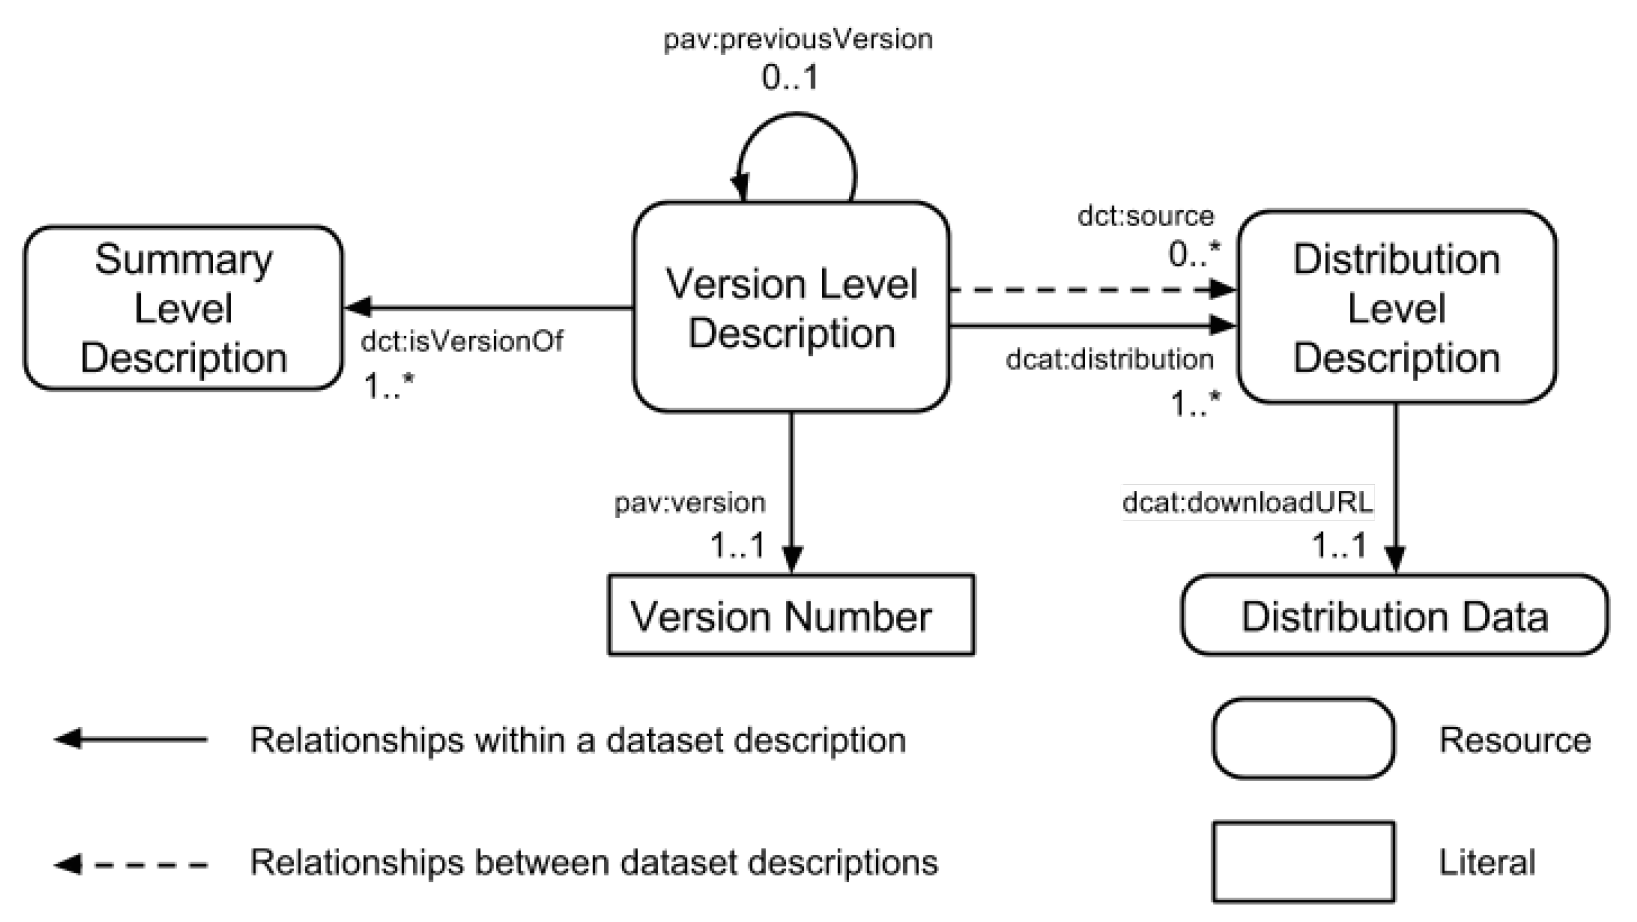
\includegraphics[scale=0.34]{figures/HCLSModel.png}
	\caption[Data model from the W3C's Health Care and Life Sciences Interest Group separating data into three levels: works, versions, and instances.]{Data model from the W3C's Health Care and Life Sciences Interest Group separating data into three levels: works, versions, and instances.  From Dummontier, et al. \cite{Dummontier2016}}
	\label{HCLSModel}
\end{figure}
The highest level summarizes the data as an abstract work, perhaps better described as a topic or title.
The data topic can have multiple versions over time.
The version can then be instantiated into various distributions with different physical formats.
The model---relating summary, version, and distribution---provides a method to implement the formation of \gls{frbr}'s work, expression, and manifestation model on the Web.

From his definition of versions, Barkstrom also outlines a hierarchical version model as seen in Figure \ref{hierarchy}.
\begin{figure}
	\centering
	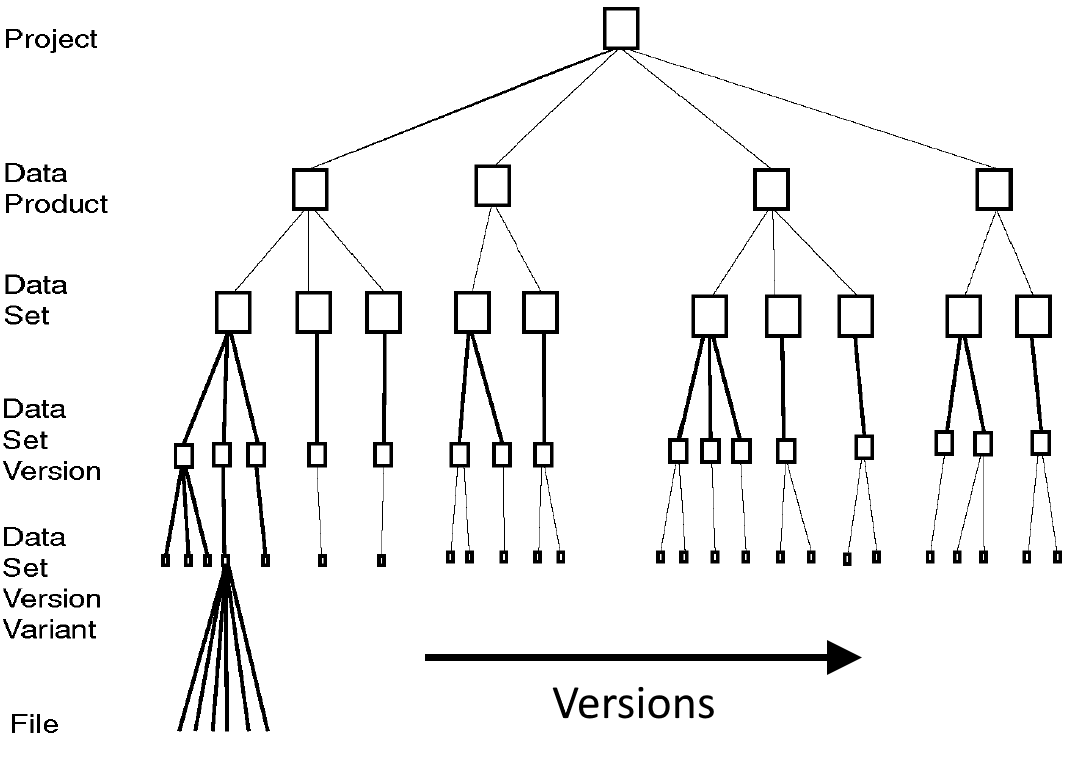
\includegraphics[scale=0.50]{figures/hierarchy.png}
	\caption[Visual representation of grouping hierarchy.]{Visual representation of grouping hierarchy.  Each row of the hierarchy defines a level of granularity where differences can separate ``homogenous groupings" of data.  From \cite{Barkstrom2003}}
	\label{hierarchy}
\end{figure}
The model features additional intermediary levels than the \gls{hcls}'s model by introducing data products and data sets as ``homogeneous groupings" where differences can be introduced \cite{barkstrom2014earth}.
Each edge in the tree signifies a difference with other objects at the same depth, but the model does not provide a mechanism to explain the difference.
The difference in the number of tiers employed in the \gls{hcls} and Barkstrom models also indicates that different applications will have varying expectations of granularity to their versioning models.
A general solution will likely need to be tiered and recursive in structure to accommodate different levels of specificity.

\section{Provenance Representation} \label{sec:provmod}

\Gls{linked} is a movement to improve data set interoperability by using technology to expose the characteristics and connections between collections of data on the Web of Data \cite{ld}.
Provenance ontologies form a major section of \gls{linked} approaches to data versioning.
The coverage stems from the close relation between provenance and differentiating versions.
The Proof Markup Language, one of the first semantic models to capture provenance information, expressed lineage relationships using inference reasoning through traceable graphs \cite{daSilva2006381}.
The technique provides a powerful way to express and imply sequences of relationships between different versions and characterize the manner of their relation.

Provenance models are a necessary step towards the development of versioning models.
Going back to the working definition of a version and the discussion from Barkstrom, \glspl{version} are produced from changes to \gls{provenance}, and without the ability to clearly trace \gls{provenance}, \glspl{version} cannot be clearly organized.
A number of \gls{linked} \gls{provenance} models include versioning concepts such as \gls{opm}, \gls{prov}, and \gls{pav}.
Each model approaches versioning differently, ranging from very broad to very narrow definitions of a \gls{version}.
None of the models approach capturing the differences between \glspl{version} which is appropriate since the differences do not explain the processes used to create a digital object \cite{moreau2008open}.
Versioning, in contrast, documents the results of using a different process.

\subsection{Open Provenance Model}

\gls{opm} was the product of a series of provenance challenges held by the International Provenance and Annotation Workshop after participants began realizing and reaching consensus on the formulation and content of provenence information necessary to establish system interoperability \cite{moreau2008open}.
In an experimental case, the model has been applied to sensor networks, automating and unifying their provenance capture even as they grow \cite{5478496}.
To aid \gls{opm}'s adoption, the framework Karma2 integrates provenance capture into scientific workflows and provides a more abstract view of their data collection activities \cite{simmhan2010karma2}.
The property \textit{opm:WasDerivedFrom} constitutes a core concept in the model and marks the reliance of one object's existence on another object.
For a large part, the relation encompasses the engagement which provenance models view versions, without further need to explore the derivation's content.

\subsection{PROV-O}\label{sec:prov}

\gls{prov}, a \gls{w3c} Recommendation, delineates a method to express data provenance in a more compact form as seen in Figure \ref{PROVO} \cite{Gil2013a} \cite{Groth2013}.
\begin{figure}
	\centering
	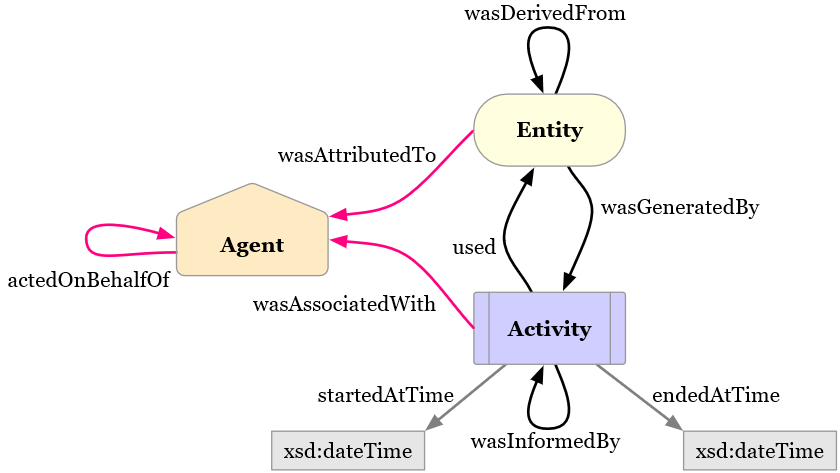
\includegraphics[scale=0.5]{figures/ProvO.png}
	\caption[Diagram of the PROV Ontology.]{The PROV Ontology is divided into three main objects: Entity, Agent, and Activity.  An Activity is an action or process which produces Entities which is associated with an Agent.  Agents are usually individuals responsible for creating Entities.  The high level ontology can capture complex provenance relationships to ensure traceability of data production.  Figure 1 from \cite{Lebo2013}}
	\label{PROVO}
\end{figure}
The recommendation uses a conceptual model relating activities, agents, and entities to describe data production lineage, the list of data ancestors leading to a data object \cite{Moreau2013c} \cite{Nies2013} \cite{Nies2013a}.
Intended as a high level abstraction, it takes an activity-oriented approach to provenance modeling.
Every data entity results from the actions of some activity \cite{Gil2013}.
The conceptual model's expression occurs through the \gls{prov} Ontology (PROV-O), which is conveyed through various resource description languages \cite{Hua2013} \cite{Klyne2013}.
The ontology is further formalized into a functional notation for easier human consumption \cite{Moreau2013b} \cite{Cheney2013a}.
One particular strength that has contributed to the adoption of \gls{prov} is its ability to link into other ontologies, making it easier for existing semantically enriched data sets to adopt \gls{prov} \cite{Miles2013} \cite{Moreau2013}.

\gls{prov} has provided a major contribution in maintaining the quality and traceability of data sets and reporting in the \gls{nca} \cite{Ma2014191}.
The inclusion into the \gls{nca} signifies that there is an increased likelihood of adoption through other scientific fields as a result of this reporting.
The Global Change Information System, which houses the data used to generate the \gls{nca}, uses \gls{prov} to meticulously track the generation of its artifacts and results as they are used in the assessment report \cite{Tilmes2012}.
The usage means that not only does the data have a traceable lineage to verify quality, but the content of documents can have the same verifiability \cite{Ma2014}.

Komadu, a framework developed to alleviate workflow integration, utilizes PROV to improve upon its predecessor, Karma, by no longer utilizing global context identifiers that were not necessarily shared throughout the workflow. \cite{Suriarachchi_2015}.
The framework and the adoption of \gls{prov} in high profile scientific applications means versioning applications can be overlayed onto a \gls{provenance} skeleton once a versioning ontology has been created.

The \gls{prov} Ontology provides three different concepts that begin to encapsulate the provenance relationship between data versions.
It defines a \textit{prov:Generation} as "the completion of production of a new entity by an activity," \cite{Lebo2013}.
This means that the generation, which corresponds adding an object to a version, must result from a \textit{prov:Activity}.
\textit{Prov:Invalidation}, defined as the, ``start of the destruction, cessation, or expiry of an existing entity by an activity," makes a similar connection between activities and entities \cite{Lebo2013}.
A third concept, \textit{prov:Derivation}, relates two entities, and the ontology defines it as, "a transformation of an entity into another, an update of an entity resulting in a new one, or the construction of a new entity based on a preexisting entity. " \cite{Lebo2013}.
PROV also has a property called \textit{prov:isDerivedFrom} which conveys the same definition as a \textit{prov:Derivation}.
Using the property and concept together forms a qualified property which can be instantiated and further annotated.

\subsection{Provenance, Authorship, and Versioning Ontology}

The \gls{pav} Ontology is, ``a lightwei\-ght vocabulary, for capturing ``just enough" descriptions essential for web resources representing digitized knowledge" \cite{Ciccarese2013}.
It provides a means to track versioning information through linked data by introducing \textit{pav:version} to cite versions and \textit{pav:previousVersion} to link them together in order \cite{Ciccarese2013}.
The authors of \gls{pav} created the new property due to a disagreement with the Dublin Core concept \textit{dc:isVersionOf} which is used when, ``Changes in version imply substantive changes in content rather than differences in format" \cite{DCMI2012}.
\gls{pav} supports the idea that a new concept becomes necessary to cover cases where new \glspl{version} do not have to be substantive but can still be alternate editions of the original object.
While it documents related versions well, \gls{pav} does not dive deeper in explaining the circumstances behind version differences.

\subsection{Schema.org}

\sloppy
The Schema.org structured data schema is not a provenance ontology but provides a means to supply searchable web pages with standardized micro-data.
The ontology has a collection of concepts which could be applied to versioning.
The \textit{schema:UpdateAction} is defined as, ``the act of managing by changing/editing the state of the object," which encompasses the same responsibilities expected of versioning systems \cite{Schema}.
The terms \textit{schema:AddAction}, \textit{schema:DeleteAction}, and \textit{schema:ReplaceAction} subclass the \textit{schema:UpdateAction}.
These classes model actions which further cement parallels between versioning and \textit{schema:UpdateAction}.

\fussy
Schema.org defines a \textit{schema:ReplaceAction} as, ``the act of editing a recipient by replacing an old object with a new object" \cite{SchemaRep}.
The concept has two properties, \textit{schema:replacee} and \textit{schema:replacer} which indicates that a new object replaces an old one.
Schema.org models the interaction by placing the replacement action at the relation's center.
In comparison, the \textit{schema:AddAction} is defined as, ``the act of editing by adding an object to a collection" \cite{SchemaAdd}.
The action only involves the object and the new state of the collection, not involving any of the collection's prior lineage.
Schema.org defines the \textit{schema:DeleteAction} as, "the act of editing a recipient by removing one of its objects," \cite{SchemaRem}.
The concept aligns well with other versioning systems, although deletion may be a strong assertion.
The term would be inappropriate for use in cases where data is archived but no longer used, for example or when data becomes deprecated.

\section{Documenting Versions} \label{sec:changelog}

When workflow activities generate new \glspl{version} of a data object, connective tissue becomes necessary to bind the \glspl{version}.
\Glspl{log}, artifacts resulting from the versioning process, play a major role filling in gaps between versions.
\Glspl{log} document changes and explain, in human language, motivations behind the differences \cite{uel1037}.
Introducing \gls{log} information into \gls{linked} follows logically from the drive to improve transparency of characteristics connecting data sets, a \gls{linked} principle.
Very little evidence exists suggesting that \gls{log} data is being captured by \gls{linked} practices.
The provenance ontologies covered in Section \ref{sec:provmod} contain terms which are too broad to express changes at the same level of detail as \glspl{log}.
\gls{nasa} Earth Science's treatment of versions has been found to vary depending on a data community's traditions, meaning that if an ontology to express change data existed, the ontology may not be applicable to every community due to opposing traditions \cite{barkstrom2014earth}.
A review of data versioning in biology also identifies the lack of a standardized versioning format suggesting the lack of an accompanying standardized method to consume versioning data.
While some data sets will contain a \gls{log}, software projects have normalized their use in version release documentation \cite{German03automatingthe}.
The popular \gls{svm} Git provides methods to attach messages to commits, but the messages are in plain-text rather than a \gls{linked} compatible format \cite{Chacon:2009:PG:1618548}.
As a result, software projects provide a basis for understanding the value of \glspl{log} to data sets with multiple \glspl{version}.
The \gls{log}'s common drawback is the limitation to only human readable text.
Wider adoption among data sets may be possible by making these texts machine computable.

The following studies demonstrate the value that can be unlocked by studying the behaviors and data stored within software \glspl{log}.
\Glspl{log} play an important communication role in open-source projects, allowing new developers to trace implementation decisions made through the life-cycle of a project.
In one project, researchers explicitly linked \gls{log} entries to documented bug reports, showing how bugs of different priorities were addressed \cite{Chen:2004:OCL:990374.990391}.
The links give insight into motivations behind particular implementation decisions.
\Glspl{log} linked with \gls{version} releases also provide feedback to the user community that issues have been addressed, in addition to ensuring that improvements drive modifications to the code base.
The rate of \gls{log} release has been shown to be a good indicator for the general health and activity within a software project \cite{German03automatingthe}.
A project mined change histories to determine dependency patterns in source code changes which would cause a cascade of follow-up bugs in other projects \cite{6132954}.
The research is pertinent to systems which rely on multiple projects to function, but also functions very similar to inter-operable data systems like those created by \gls{linked}.
The change history mining project diverges from previous approaches by looking primarily at the presence of differences between the source code instead of the natural language text in accompanying logs.

\section{The Versioning Use Case} \label{sec:usecase}

The research questions addressed by this thesis revolve around the check and retrieval stages of the flow in the Versioning Use Case shown in Table \ref{table:UseCase}.
\begin{table}
	\caption{Versioning Use Case Table}
	\label{table:UseCase}
	\centering
	\begin{tabular}{|L{14cm}|}
		\hline
		\textbf{Use Case Name}: New Version Publication \& Retrieval\\
		\hline
		\textbf{Goal}: Record a new version of a data set and provide it to a data consumer.\\
		\hline
		\textbf{Summary}: The Producer creates a new version of their data and must record it to the Versioning System while providing the Consumer with the data\\
		\hline
		\textbf{Actors}: Producer, Consumer\\
		\hline
		\textbf{Preconditions}: Producer has supplied some data to the Versioning System.   Consumer has retrieved the data from the Versioning System.\\
		\hline
		\textbf{Triggers}: Producer provides a different version of the data to the Versioning System.\\
		\hline
		\textbf{Basic Flow}: 
		\begin{enumerate}
			\item Producer places the next version into the Versioning System.
			\item Producer may repeat the previous action 0 or more times.
			\item Consumer checks the data to see if there are changes.
			\item If there are pertinent changes:
			\begin{enumerate}
				\item Consumer retrieves the updated data.
			\end{enumerate}
		\end{enumerate}\\
		\hline
		\textbf{Alternate Flow}:
		\begin{enumerate}
			\item Producer places the next version into the Versioning System.
			\item Producer notifies Consumer that an alternate version is available.
			\item Consumer retrieves the updated data.
		\end{enumerate}\\
		\hline
		\textbf{Post Conditions}: Producer has made the alternate version available.  Consumer possesses the pertinent newly available version.\\
		\hline
	\end{tabular}
\end{table}
The goal of the Versioning Use Case is to allow the data producer to communicate changes of data tracked by the versioning system to the data consumer.
The use case begins when a data producer wishes to distribute the next \gls{version} of a data set.
While \glspl{version} for observations of phenomena are sequential, alternate \glspl{version} can deal with older data or occur concurrently with the object the alternate changes so the adjective new or newer is avoided when possible.
The use case features the data producer and data consumer as actors using the versioning system as an intermediary.
The actors do not follow separate use cases because each actor relies on the actions of the other actor to contextualize the actions in the use case.

The basic flow of the use case is seen in Figure \ref{UCD1} where the producer logs a version into the versioning system, and the consumer retrieves that data version.
\begin{figure}
	\centering
	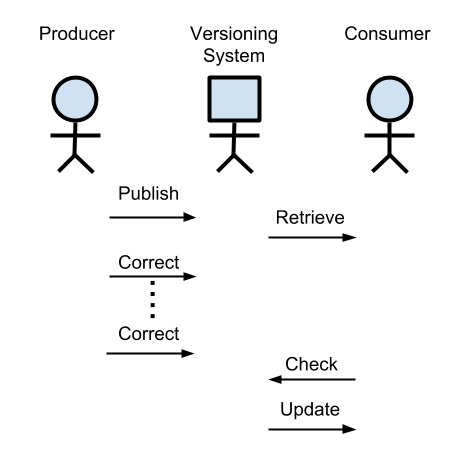
\includegraphics[scale=1]{figures/UC_Diagram1.png}
	\caption[Versioning Use Case Basic Flow]{Basic Flow of the Versioning Use Case.  The data producer adds a data set to be tracked by the versioning system.  After the data consumer retrieves the data, the producer makes a series of updates and corrections to the original data.  The consumer then returns to determine if there are changes to pertinent data files.  The consumer then updates as necessary.}
	\label{UCD1}
\end{figure}
At a later point in time, the producer can add any number of corrections to the versioning system.
The repeated corrections reflect a practice of passively logging additional changes.
At some final time after 0 or more corrections, the Consumer returns to check the versioning system for any changes to the data set the Consumer retrieved.
If there are changes to parts pertinent to the Consumer, the actor retrieves the corrected data.
In the interaction, the Producer only passively provides additional versions of the data while the responsibility of remaining up-to-date lies with the Consumer.
The ability of the  versioning system to communicate to the Consumer that the data has changed determines whether the use case succeeds or fails for the data consumer.
The relationship creates a Producer/Consumer dynamic which influences the performance of the versioning system.

The alternate flow in Figure \ref{UCD2} requires additional information from the Consumer which is a means of notification.
\begin{figure}
	\centering
	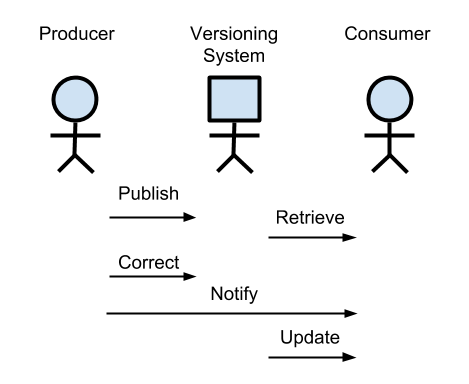
\includegraphics[scale=1]{figures/UC_Diagram2.png}
	\caption[Versioning Use Case Alternate Flow]{In the alternate flow, the authority to determine necessary updates lies with the producer.  After correcting data tracked by the versioning system, the producer notifies the consumer to update the consumer's data.}
	\label{UCD2}
\end{figure}
The flow begins the same as the basic flow, but after a single correction, the Producer notifies the Consumer that the data has changed.
The notification causes the Consumer to come and retrieve the updated data set.
The alternate flow poses a few problems in that the Producer must now manage notification information, but the Producer must also notify all consumers of the data which may cause scalability issues.
Notice that in both flows, the data Producer possesses the authority to determine change through data publication.
The data Consumer only takes from the versioning system except in step three of the basic flow.
It is only when the Consumer checks the \glspl{version} in the system or is notified by the Producer that the Consumer can contextualize changes to the retrieved data set.

\subsection{Research Question 1: What has changed?}

The primary research question addressed in the following chapters pertains to step three in the basic flow of the use case.
In order to execute step three, the Consumer must have a means of determining whether the data set is different from the one the Consumer currently possesses.
In a large number of software projects, especially open-source projects, \glspl{log} document for the producer changes to the code base and communicate alterations to the Consumer.
Very few data sets provide detailed \glspl{log} along with \glspl{version} in the versioning system.
Either general descriptions of changes are made or new documentation explaining usage is provided, requiring the data consumer to manually acclimate to changes.

The prevailing approach to addressing Research Question 1 is that automating the generation of \glspl{log} will allow the addition of \gls{linked} into \gls{log} content.
To encode changes as \gls{linked}, I developed a versioning ontology called \gls{vo}
The additional data allows data consumers the ability to search, filter, and otherwise interact with change information.
Different standards exist across various national agencies, but few fundamentals have been established on what needs to be included and how the information is to be captured or presented.
I determine whether a linked data versioning model would provide a standardized basis for discussing version change as well as allow tools to be developed to assist in step three for large data sets of which Consumers may only use a part.

\subsection{Research Question 2: How much has changed?}

A follow-up query to Research Question 1 is that once the changes have been determined, Consumers need to evaluate the impact of the changes.
As previously mentioned, Producers sequentially label \glspl{version} to communicate change, but many have adopted the practice of using decimals or dots to imply fractional changes, forming a dot-decimal identifier.
The authority to determine the magnitude of change lies with the Producer since the label must be applied at publication.
Version counts, as shown in Chapter \ref{ch:graph}, provide a very bland description of the changes in a version by aggregating a range of changes under a sequential label.
Using \gls{vo}, the changes can be broken down into \gls{AIM} classifications which provide a more encapsulating description of a version transition.
I test whether the AIM change counts would tie change metrics back to data differences rather than to versions.
I determine whether the AIM changes also provide a means to compare the difference between the amount of change declared by the Producer and quantity of change as seen by various Consumers.

\subsection{Research Question 3: How fast does the data change?}

Once a standardized metric for determining \gls{changedist} has been determined, assessing change rate logically follows.
Up to this point, evaluating the differences between versions has been discussed without respect to time.
Notice from the Versioning Use Case that the Producer has the ability to control the rate of version release by determining when to push corrections into the versioning system, meaning the time between \glspl{version} is not required to be consistent.
Variable release times allows the Producer to control the data volatility, the likelihood of a data set to change, by aggregating changes over time.
Without considering time, \gls{changedist} across \glspl{version} misrepresents the actual change rate of a data set.
Looking at just the version publication rate also misrepresents the actual change rate of a data set since total change can vary between \glspl{version}.
I hypothesize that version analysis needs to factor in time when comparing change rates between \glspl{version}.
The change rate distribution of each \gls{AIM} \gls{change} follow a distribution significantly different from the version publication rate.

\section{Hypothesis Statement}

The work in this dissertation tests five hypotheses.
In the first hypothesis, using the versioning model \gls{vo} to expose \glspl{log} as \gls{linked} creates a standardized basis for discussing versioning as well as allow tools to assist in versioning analysis.
\gls{vo} improves upon current versioning concepts in provenance models with more precise semantics and a focus on version differences rather than version genesis.
The ontology and the corresponding model assume that at least two \glspl{version} are necessary to conduct versioning activities, meaning data sets with one \gls{version} cannot be captured.
A method to address the limitation is to introduce a dummy or empty \gls{version}, but the approach is not explored because it skews the change metric towards new \gls{add}.
\gls{vo} was applied at the data set granularity to ensure that the detected differences are less abstract and more traceable, to ensure that differences don't result from differences in instrumentation or projects for example.

The second and third hypotheses tests the suitability of \gls{AIM} change counts as a metric to measure \gls{change} between \glspl{version}.
The second hypothesis determines whether \gls{AIM} counts improve upon the current practice by capturing data differences rather than the sequential labeling common to many versioning traditions.
The counts are collected from a \gls{vergraph} constructed with \gls{vo} using \gls{rdf} triples.
Because version graphs will catalog individual changes, a count based on the different types of changes are expected to produce a more revealing change metric.
The metric can be verified by comparison with the amount of change indicated by the version identifier assigned by the producer.
Hypothesis two also shows a method to compare within a particular kind of change---\gls{add}, \gls{invalidate}, or \gls{modify}---through subclassing concepts within \gls{vo}.
The third hypothesis states that \gls{AIM} counts provide a method to compare the amount of change as seen by various data consumers.

Hypothesis four and five test the effect of time on change counts.
The analysis to evaluate hypothesis two and three rely only the differences between \glspl{version} but do not consider how the \glspl{version} are distributed across time.
Hypothesis four considers whether computing \gls{changedist} without time misrepresents the actual change rate.
Because \glspl{change} cannot be computed until a version publication, the total change count is distributed over the valid duration of the previous \gls{version}.
The \glspl{change} computed are assumed to be aggregated from the publication of the previous \gls{version}.
Hypothesis five states that the distribution change rate of data sets is significantly different from the publication rate of versions.
The evaluation of hypothesis five will determine whether version publication rate is a representative proxy for the actual change rate.

\section{Contributions}

%Add chapter number and references.

In Chapter \ref{ch:model}, I present my first contribution, the model forming the basis of \gls{vo} which is used to instantiate \glspl{vergraph}.
\Glspl{vergraph} capture differences between objects, not the course used to create a data object, differentiating themselves from provenance graphs.
The \gls{vergraph} enables my second contribution, a standardized process to compute and publish \gls{linked} \glspl{log}, covered in Chapter \ref{ch:changelog}.
The contribution eases consuming very lengthy logs, which data sets often produce, as well as enabling searchability and discoverability of \glspl{change} affecting the \gls{version}.
My third contribution, discussed in Chapter \ref{ch:graph}, is using a \gls{vergraph} to provide a quantitative metric for determining \gls{changedist}.
Differing methods between data producers and consumers in computing \gls{changedist} highlights disagreements in the prodcuer/consumer dynamic.
A fourth contribution is a comparison between version publication and change rates, found in Chapter \ref{Volatility}, to determine the propriety of versions as proxies for change.

%%% Local Variables:
%%% mode: latex
%%% TeX-master: t
%%% End:
